\documentclass[tikz,border=8pt]{standalone}
\usepackage{amsmath,amssymb}
\usepackage{tikz}
\usetikzlibrary{decorations.pathreplacing,arrows.meta,calc,patterns}

\begin{document}
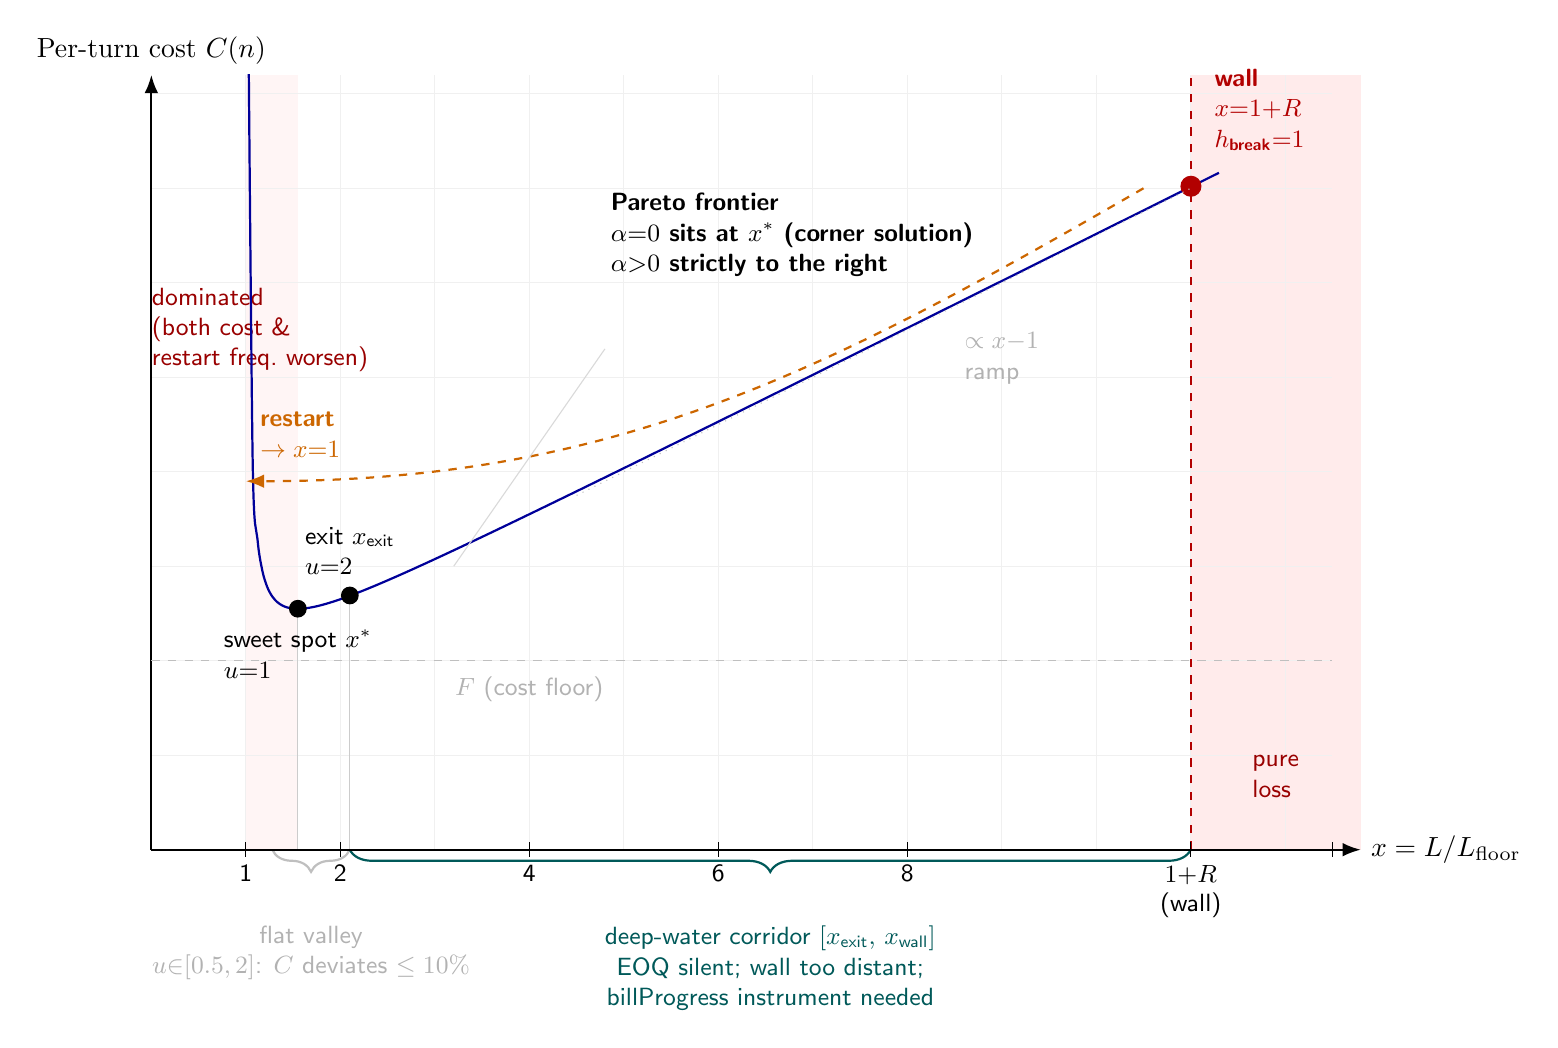
\begin{tikzpicture}[
  scale=1.2,
  >=Latex,
  annot/.style={font=\small\sffamily,align=left},
  boldannot/.style={font=\small\sffamily\bfseries,align=left},
  gridstyle/.style={gray!12,thin},
]

% ===================================================================
% LAYER 1: Background fills (behind everything)
% ===================================================================
\fill[red!4] (1.0,0) rectangle (1.55,8.2);
\fill[red!8] (11.0,0) rectangle (12.8,8.2);

% ===================================================================
% LAYER 2: Grid & structural guides (behind axes)
% ===================================================================
\foreach \x in {0,...,12} { \draw[gridstyle] (\x,0) -- (\x,8.2); }
\foreach \y in {0,...,8}   { \draw[gridstyle] (0,\y) -- (12.5,\y); }

% Vertical drop lines (end at x-axis; axes drawn on top for clean join)
\draw[gray!40,thin] (1.55, 2.55) -- (1.55,0);   % sweet spot
\draw[gray!40,thin] (2.1, 2.69)  -- (2.1,0);     % exit

% Wall dashed line
\draw[red!70!black,thick,dashed] (11.0,0) -- (11.0,8.2);

% Braces — baseline on x-axis, axes drawn on top afterward
\draw[decorate,decoration={brace,mirror,amplitude=8pt},gray!50,thick]
  (1.28,0) -- (2.10,0);
\draw[decorate,decoration={brace,mirror,amplitude=8pt},teal!70!black,thick]
  (2.1,0) -- (11.0,0);

% ===================================================================
% LAYER 3: Axes (on top of lines/braces at y=0 — clean, unbroken)
% ===================================================================
\draw[->,thick] (0,0) -- (0,8.2) node[above] {Per-turn cost $C(n)$};
\draw[->,thick] (0,0) -- (12.8,0) node[right] {$x = L/L_{\text{floor}}$};

% x-axis tick marks
\foreach \x/\l in {1/1, 2/2, 4/4, 6/6, 8/8, 11/\shortstack{$1{+}R$\\(wall)}, 12.5/} {
  \draw (\x,0.08) -- (\x,-0.08);
  \node[annot,below=2pt] at (\x,0) {\l};
}

% ===================================================================
% LAYER 4: Fill region text
% ===================================================================
\node[annot,red!60!black] at (1.15,5.5) {dominated\\(both cost \&\\restart freq.\ worsen)};
\node[annot,red!60!black,anchor=south] at (11.9,0.45) {pure\\loss};

% ===================================================================
% LAYER 5: Curve, data points, annotations (above axes)
% ===================================================================
% Scope with clip so left arm stays inside the axis box
\begin{scope}
\clip (0,0) rectangle (12.8,8.2);
\draw[thick,blue!60!black,domain=1.02:11.3,smooth,variable=\x,samples=200]
  plot ({\x}, {0.151/(\x-1) + 2.0 + 0.50*(\x-1)});
\end{scope}

% Floor line
\draw[dashed,gray!50,thin] (0,2.0) -- (12.5,2.0);
\node[annot,gray!60] at (4.0,1.7) {$F$ (cost floor)};

% Sweet spot — label BELOW the point
\coordinate (sweet) at (1.55, 2.55);
\filldraw[black] (sweet) circle (2.5pt);
\node[annot,below=4pt] at (sweet) {sweet spot $x^*$\\$u{=}1$};

% Exit — label ABOVE the point
\coordinate (exit) at (2.1, 2.69);
\filldraw[black] (exit) circle (2.5pt);
\node[annot,above=4pt] at (exit) {exit $x_{\text{exit}}$\\$u{=}2$};

% Wall point
\coordinate (wallpt) at (11.0, 7.02);
\filldraw[red!70!black] (wallpt) circle (3pt);
\node[boldannot,red!70!black,anchor=south west] at (11.15,7.3) {wall\\$x{=}1{+}R$\\$h_{\text{break}}{=}1$};

% Flat valley annotation text
\node[annot,gray!60,below=24pt,align=center] at (1.69,0)
  {flat valley\\$u{\in}[0.5,2]$: $C$ deviates $\le 10\%$};

% Deep-water corridor annotation text
\node[annot,teal!70!black,below=24pt,text width=6.5cm,align=center] at (6.55,0)
  {deep-water corridor $[x_{\text{exit}},\,x_{\text{wall}}]$\\EOQ silent; wall too distant; billProgress instrument needed};

% Restart arrow
\draw[->,orange!80!black,thick,dashed] (10.5,7.0) to[out=210,in=0] (1.0,3.9);
\node[boldannot,orange!80!black,anchor=south west] at (1.05,4.05) {restart\\$\rightarrow x{=}1$};

% Pareto frontier annotation
\node[boldannot,anchor=south west,inner sep=2pt] at (4.8,6.0)
  {Pareto frontier\\$\alpha{=}0$ sits at $x^*$ (corner solution)\\$\alpha{>}0$ strictly to the right};
\draw[gray!30,thin] (4.8,5.3) -- (3.2,3.0);

% Slope ghost line
\draw[gray!50,dotted,thin,domain=4.5:11.0,smooth,variable=\x]
  plot ({\x}, {0.50*(\x-1) + 2.0});
\node[annot,gray!60] at (9.0,5.2) {$\propto x{-}1$\\ramp};

\end{tikzpicture}
\end{document}
